%!TEX root = ../../thesis.tex
\section{Real Computability Theory}\label{sec:real computability}
\subsection{Classical Computability Theory}
 \begin{figure}[h]
   \centering
   %% Graphic for TeX using PGF
% Title: /home/holger/git/dotfiles/Diagram1.dia
% Creator: Dia v0.97.2
% CreationDate: Thu Mar 26 15:54:30 2015
% For: holger
% \usepackage{tikz}
% The following commands are not supported in PSTricks at present
% We define them conditionally, so when they are implemented,
% this pgf file will use them.
\ifx\du\undefined
  \newlength{\du}
\fi
\setlength{\du}{10\unitlength}
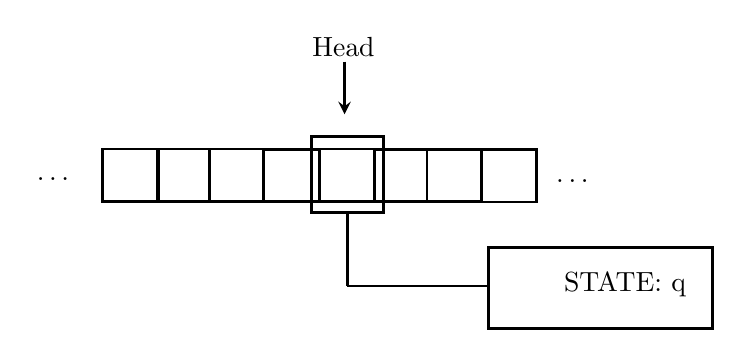
\begin{tikzpicture}
\pgftransformxscale{1.000000}
\pgftransformyscale{-1.000000}
\definecolor{dialinecolor}{rgb}{0.000000, 0.000000, 0.000000}
\pgfsetstrokecolor{dialinecolor}
\definecolor{dialinecolor}{rgb}{1.000000, 1.000000, 1.000000}
\pgfsetfillcolor{dialinecolor}
\definecolor{dialinecolor}{rgb}{1.000000, 1.000000, 1.000000}
\pgfsetfillcolor{dialinecolor}
\fill (18.550000\du,8.550000\du)--(18.550000\du,10.450000\du)--(20.550000\du,10.450000\du)--(20.550000\du,8.550000\du)--cycle;
\pgfsetlinewidth{0.100000\du}
\pgfsetdash{}{0pt}
\pgfsetdash{}{0pt}
\pgfsetmiterjoin
\definecolor{dialinecolor}{rgb}{0.000000, 0.000000, 0.000000}
\pgfsetstrokecolor{dialinecolor}
\draw (18.550000\du,8.550000\du)--(18.550000\du,10.450000\du)--(20.550000\du,10.450000\du)--(20.550000\du,8.550000\du)--cycle;
% setfont left to latex
\definecolor{dialinecolor}{rgb}{0.000000, 0.000000, 0.000000}
\pgfsetstrokecolor{dialinecolor}
\node at (19.550000\du,9.695000\du){};
\definecolor{dialinecolor}{rgb}{1.000000, 1.000000, 1.000000}
\pgfsetfillcolor{dialinecolor}
\fill (20.565000\du,8.555000\du)--(20.565000\du,10.455000\du)--(22.565000\du,10.455000\du)--(22.565000\du,8.555000\du)--cycle;
\pgfsetlinewidth{0.100000\du}
\pgfsetdash{}{0pt}
\pgfsetdash{}{0pt}
\pgfsetmiterjoin
\definecolor{dialinecolor}{rgb}{0.000000, 0.000000, 0.000000}
\pgfsetstrokecolor{dialinecolor}
\draw (20.565000\du,8.555000\du)--(20.565000\du,10.455000\du)--(22.565000\du,10.455000\du)--(22.565000\du,8.555000\du)--cycle;
% setfont left to latex
\definecolor{dialinecolor}{rgb}{0.000000, 0.000000, 0.000000}
\pgfsetstrokecolor{dialinecolor}
\node at (21.565000\du,9.700000\du){};
\definecolor{dialinecolor}{rgb}{1.000000, 1.000000, 1.000000}
\pgfsetfillcolor{dialinecolor}
\fill (22.415000\du,8.555000\du)--(22.415000\du,10.455000\du)--(24.415000\du,10.455000\du)--(24.415000\du,8.555000\du)--cycle;
\pgfsetlinewidth{0.100000\du}
\pgfsetdash{}{0pt}
\pgfsetdash{}{0pt}
\pgfsetmiterjoin
\definecolor{dialinecolor}{rgb}{0.000000, 0.000000, 0.000000}
\pgfsetstrokecolor{dialinecolor}
\draw (22.415000\du,8.555000\du)--(22.415000\du,10.455000\du)--(24.415000\du,10.455000\du)--(24.415000\du,8.555000\du)--cycle;
% setfont left to latex
\definecolor{dialinecolor}{rgb}{0.000000, 0.000000, 0.000000}
\pgfsetstrokecolor{dialinecolor}
\node at (23.415000\du,9.700000\du){};
\definecolor{dialinecolor}{rgb}{1.000000, 1.000000, 1.000000}
\pgfsetfillcolor{dialinecolor}
\fill (24.380000\du,8.560000\du)--(24.380000\du,10.460000\du)--(26.380000\du,10.460000\du)--(26.380000\du,8.560000\du)--cycle;
\pgfsetlinewidth{0.100000\du}
\pgfsetdash{}{0pt}
\pgfsetdash{}{0pt}
\pgfsetmiterjoin
\definecolor{dialinecolor}{rgb}{0.000000, 0.000000, 0.000000}
\pgfsetstrokecolor{dialinecolor}
\draw (24.380000\du,8.560000\du)--(24.380000\du,10.460000\du)--(26.380000\du,10.460000\du)--(26.380000\du,8.560000\du)--cycle;
% setfont left to latex
\definecolor{dialinecolor}{rgb}{0.000000, 0.000000, 0.000000}
\pgfsetstrokecolor{dialinecolor}
\node at (25.380000\du,9.705000\du){};
\definecolor{dialinecolor}{rgb}{1.000000, 1.000000, 1.000000}
\pgfsetfillcolor{dialinecolor}
\fill (26.415000\du,8.555000\du)--(26.415000\du,10.455000\du)--(28.415000\du,10.455000\du)--(28.415000\du,8.555000\du)--cycle;
\pgfsetlinewidth{0.100000\du}
\pgfsetdash{}{0pt}
\pgfsetdash{}{0pt}
\pgfsetmiterjoin
\definecolor{dialinecolor}{rgb}{0.000000, 0.000000, 0.000000}
\pgfsetstrokecolor{dialinecolor}
\draw (26.415000\du,8.555000\du)--(26.415000\du,10.455000\du)--(28.415000\du,10.455000\du)--(28.415000\du,8.555000\du)--cycle;
% setfont left to latex
\definecolor{dialinecolor}{rgb}{0.000000, 0.000000, 0.000000}
\pgfsetstrokecolor{dialinecolor}
\node at (27.415000\du,9.700000\du){};
\definecolor{dialinecolor}{rgb}{1.000000, 1.000000, 1.000000}
\pgfsetfillcolor{dialinecolor}
\fill (28.380000\du,8.560000\du)--(28.380000\du,10.460000\du)--(30.380000\du,10.460000\du)--(30.380000\du,8.560000\du)--cycle;
\pgfsetlinewidth{0.100000\du}
\pgfsetdash{}{0pt}
\pgfsetdash{}{0pt}
\pgfsetmiterjoin
\definecolor{dialinecolor}{rgb}{0.000000, 0.000000, 0.000000}
\pgfsetstrokecolor{dialinecolor}
\draw (28.380000\du,8.560000\du)--(28.380000\du,10.460000\du)--(30.380000\du,10.460000\du)--(30.380000\du,8.560000\du)--cycle;
% setfont left to latex
\definecolor{dialinecolor}{rgb}{0.000000, 0.000000, 0.000000}
\pgfsetstrokecolor{dialinecolor}
\node at (29.380000\du,9.705000\du){};
\definecolor{dialinecolor}{rgb}{1.000000, 1.000000, 1.000000}
\pgfsetfillcolor{dialinecolor}
\fill (30.280000\du,8.560000\du)--(30.280000\du,10.460000\du)--(32.280000\du,10.460000\du)--(32.280000\du,8.560000\du)--cycle;
\pgfsetlinewidth{0.100000\du}
\pgfsetdash{}{0pt}
\pgfsetdash{}{0pt}
\pgfsetmiterjoin
\definecolor{dialinecolor}{rgb}{0.000000, 0.000000, 0.000000}
\pgfsetstrokecolor{dialinecolor}
\draw (30.280000\du,8.560000\du)--(30.280000\du,10.460000\du)--(32.280000\du,10.460000\du)--(32.280000\du,8.560000\du)--cycle;
% setfont left to latex
\definecolor{dialinecolor}{rgb}{0.000000, 0.000000, 0.000000}
\pgfsetstrokecolor{dialinecolor}
\node at (31.280000\du,9.705000\du){};
\definecolor{dialinecolor}{rgb}{1.000000, 1.000000, 1.000000}
\pgfsetfillcolor{dialinecolor}
\fill (32.245000\du,8.565000\du)--(32.245000\du,10.465000\du)--(34.245000\du,10.465000\du)--(34.245000\du,8.565000\du)--cycle;
\pgfsetlinewidth{0.100000\du}
\pgfsetdash{}{0pt}
\pgfsetdash{}{0pt}
\pgfsetmiterjoin
\definecolor{dialinecolor}{rgb}{0.000000, 0.000000, 0.000000}
\pgfsetstrokecolor{dialinecolor}
\draw (32.245000\du,8.565000\du)--(32.245000\du,10.465000\du)--(34.245000\du,10.465000\du)--(34.245000\du,8.565000\du)--cycle;
% setfont left to latex
\definecolor{dialinecolor}{rgb}{0.000000, 0.000000, 0.000000}
\pgfsetstrokecolor{dialinecolor}
\node at (33.245000\du,9.710000\du){};
% setfont left to latex
\definecolor{dialinecolor}{rgb}{0.000000, 0.000000, 0.000000}
\pgfsetstrokecolor{dialinecolor}
\node[anchor=west] at (19.550000\du,9.500000\du){};
\pgfsetlinewidth{0.100000\du}
\pgfsetdash{}{0pt}
\pgfsetdash{}{0pt}
\pgfsetmiterjoin
\definecolor{dialinecolor}{rgb}{0.000000, 0.000000, 0.000000}
\pgfsetstrokecolor{dialinecolor}
\draw (26.100000\du,8.100000\du)--(26.100000\du,10.850000\du)--(28.700000\du,10.850000\du)--(28.700000\du,8.100000\du)--cycle;
% setfont left to latex
\definecolor{dialinecolor}{rgb}{0.000000, 0.000000, 0.000000}
\pgfsetstrokecolor{dialinecolor}
\node at (27.400000\du,9.670000\du){};
\pgfsetlinewidth{0.100000\du}
\pgfsetdash{}{0pt}
\pgfsetdash{}{0pt}
\pgfsetbuttcap
{
\definecolor{dialinecolor}{rgb}{0.000000, 0.000000, 0.000000}
\pgfsetfillcolor{dialinecolor}
% was here!!!
\pgfsetarrowsend{stealth}
\definecolor{dialinecolor}{rgb}{0.000000, 0.000000, 0.000000}
\pgfsetstrokecolor{dialinecolor}
\draw (27.300000\du,5.400000\du)--(27.300000\du,7.300000\du);
}
% setfont left to latex
\definecolor{dialinecolor}{rgb}{0.000000, 0.000000, 0.000000}
\pgfsetstrokecolor{dialinecolor}
\node[anchor=west] at (27.900000\du,5.000000\du){};
% setfont left to latex
\definecolor{dialinecolor}{rgb}{0.000000, 0.000000, 0.000000}
\pgfsetstrokecolor{dialinecolor}
\node[anchor=west] at (25.750000\du,4.850000\du){Head};
\pgfsetlinewidth{0.100000\du}
\pgfsetdash{}{0pt}
\pgfsetdash{}{0pt}
\pgfsetbuttcap
{
\definecolor{dialinecolor}{rgb}{0.000000, 0.000000, 0.000000}
\pgfsetfillcolor{dialinecolor}
% was here!!!
\definecolor{dialinecolor}{rgb}{0.000000, 0.000000, 0.000000}
\pgfsetstrokecolor{dialinecolor}
\draw (27.400000\du,10.850000\du)--(27.400000\du,13.500000\du);
}
\pgfsetlinewidth{0.100000\du}
\pgfsetdash{}{0pt}
\pgfsetdash{}{0pt}
\pgfsetbuttcap
{
\definecolor{dialinecolor}{rgb}{0.000000, 0.000000, 0.000000}
\pgfsetfillcolor{dialinecolor}
% was here!!!
\definecolor{dialinecolor}{rgb}{0.000000, 0.000000, 0.000000}
\pgfsetstrokecolor{dialinecolor}
\draw (27.400000\du,13.500000\du)--(32.450000\du,13.500000\du);
}
\definecolor{dialinecolor}{rgb}{1.000000, 1.000000, 1.000000}
\pgfsetfillcolor{dialinecolor}
\fill (32.500000\du,12.100000\du)--(32.500000\du,15.050000\du)--(40.600000\du,15.050000\du)--(40.600000\du,12.100000\du)--cycle;
\pgfsetlinewidth{0.100000\du}
\pgfsetdash{}{0pt}
\pgfsetdash{}{0pt}
\pgfsetmiterjoin
\definecolor{dialinecolor}{rgb}{0.000000, 0.000000, 0.000000}
\pgfsetstrokecolor{dialinecolor}
\draw (32.500000\du,12.100000\du)--(32.500000\du,15.050000\du)--(40.600000\du,15.050000\du)--(40.600000\du,12.100000\du)--cycle;
% setfont left to latex
\definecolor{dialinecolor}{rgb}{0.000000, 0.000000, 0.000000}
\pgfsetstrokecolor{dialinecolor}
\node at (36.550000\du,13.770000\du){};
% setfont left to latex
\definecolor{dialinecolor}{rgb}{0.000000, 0.000000, 0.000000}
\pgfsetstrokecolor{dialinecolor}
\node[anchor=west] at (34.850000\du,13.455000\du){STATE: q};
% setfont left to latex
\definecolor{dialinecolor}{rgb}{0.000000, 0.000000, 0.000000}
\pgfsetstrokecolor{dialinecolor}
\node[anchor=west] at (15.800000\du,9.650000\du){$\dots$};
% setfont left to latex
\definecolor{dialinecolor2}{rgb}{0.000000, 0.000000, 0.000000}
\pgfsetstrokecolor{dialinecolor2}
\node[anchor=west] at (34.565000\du,9.700000\du){$\dots$};
\end{tikzpicture}

   \caption{A Turing-machine consists of an infinite tape with symbols from
   $\Sigma$. The head is positioned on top of one tape cell.}
 \end{figure}
 Since in real computability theory many aspects of classical computability theory are extended, 
 a very brief overview is given in the following section. 
 A detailed introduction can for example be found in \cite{computability}

 To define computability the Turing-Machine model is used.
 The Turing-Machine was invented by Alan Turing in 1936 \cite{Turing} and can
 be seen as simplified mathematical model for a computer.

 The machine consists of an infinite tape that is divided into cells. 
 Each cell contains exactly one symbol from a predefined finite alphabet
 $\Sigma$.
 It further consists of a head that is always positioned on top of one cell 
 and can in one step read and write the content of the cell and then move one
 cell left or right on the tape.

 The machine is always in one of finitely many states and has a finite
 instruction table containing instructions of the form when in state $q$ and
 reading symbol $s$, write $s'$ and move head to the left (or to the right).

 A formal definition can for example be found in \cite{Hopmann}.
 
 \begin{definition}
 	A possibly partial function $f:\subseteq \Sigma^* \to \Sigma^*$ is called \textbf{computable} if there exists 
 	a Turing-Machine, so that for all $x \in dom(f)$ the machine terminates after finitely many steps with $f(x)$ on its 
 	tape and for $x \not \in dom(f)$ the machine does not terminate.
 \end{definition}

 Even tough the Turing-Machine model is quite simple, it can be used to
 simulate every computer algorithm.
 The widely believed \textbf{Church-Turing thesis} even states, that anything
 that is computable in an informal sense, can be computed with a
 Turing-machine.

 The following definitions for sets also play a very important role in
 computability theory.
  \begin{definition}
A set $A \subseteq \Sigma^*$ is called \textbf{decidable}, if its characteristic function is computable.
\end{definition}
\begin{definition}
A set $A \subseteq \Sigma^*$ is called \textbf{recursively enumerable} (r.e.) or \textbf{computably enumerable} (c.e.) if
it is empty or if $A$ is the domain of a computable function.
\end{definition}
\subsection{Computability of real numbers}
The previous section showed how to define computability for functions over finite alphabets $\Sigma^* \to \Sigma^*$. 
That is enough to define computability for finite structures, but does not
suffice to make any statements on real numbers.

The following section defines how to extend the classical notion to uncountable
objects such as real or complex numbers, functions or infinite sequences.

There are several non equivalent ways, to define computability on such objects. 
In contrast to the classical case, where the definition using Turing-machines is widely accepted, there is no 
generally accepted model for real complexity theory.

One possible model is the so called \textbf{Type 2 Theory of Effectivity}
(TTE). \cite{Weihrauch} 
This model aims to realistically model what is possible to compute with a
computer and is useful in the analysis of the algorithms that will follow
later.
It is therefore the sole model used in this thesis. 

TTE extends the Turing-Machine model to so called type-2 Turing-machines, that
can work on infinite strings $s \in \Sigma^w$. 
\begin{definition}
A type-2 Turing-machine is a multi-tape Turing-machine with two special tapes,
an \textbf{input tape} and an \textbf{output tape}, and at least one working
tape. 
The input tape is read-only, i.e. it is not possible to change a cell on the
tape. Further, the head on both input and output tape can not be moved to the
left. In particular it is not possible to change a symbol that has been written
on the output tape once. 
\end{definition}
From now on the term Turing-Machine is used both for classical and type 2
machines, when it is obvious by context which model is meant.
\begin{definition}\label{def:computability_ttt}
A function $F:\subseteq \Sigma^\omega \to \Sigma^\omega$ is called computable if there is a Turing-Machine  
that for each infinite strings $\sigma in dom(F)$ on its input tape, writes the infinite string $F(\sigma)$ on its output tape. 
For $\sigma \not \in dom(f)$ the machine writes only finitely many symbols on the output tape.  
\end{definition}
To talk about computability over some arbitrary set, it has to be encoded to
$\sigma^\omega$. 
Such an encoding can be formalized in the following way
\begin{definition}\label{def:representation}
	A \textbf{representation} of a set $X$ is a partial surjective mapping $\alpha: \sigma^\omega \to X$. \\
	$\bar \sigma \in \alpha^{-1}(\sigma)$ is called an \textbf{$\alpha$-name} of $\sigma$. \\
	$x \in X$ is \textbf{$\alpha$-computable} if it has a decidable $\alpha$-name.
\end{definition}

In contrast to the countable case, where a canonical encoding is obvious in most
cases, finding a good representation is more challenging in the uncountable
case.
Different representations can lead to a different computability notion.
Thus it is important to find a representation that leads to a useful and
realistic notion of computability.

Some possible representations for real numbers are as follows
\begin{enumerate}
\item A $\rho_{10}$-name of $x$ is the usual decimal expansion of $x$.
\item A $\rho$-name of $x \in \RR$ is a sequence $a_n \in \ZZ$ s.t. $| x - a_n | \leq 2^{-n}$
\item  A $\rho_C$-name of $x \in \RR$ consists of two sequences rational $(q_n)_{n \in \NN}$ and $(\varepsilon_n)_{n \in \NN}$, so that 
$| x_n - q_n | < \varepsilon_n$ and $\lim_{n \to \infty} \varepsilon_n = 0$  
\item $\rho_<$-name, $\rho_>$-name
\item $\rho_n$-name 
\end{enumerate}
Some of the above notions lead to an equivalent definition of a computable real
numbers, but others do not.

In particular the following are equivalent
\begin{theorem}
\begin{enumerate}
  \item $x \in \RR$ is computable in the sense of Definition 
  \item $x \in \RR$ is $\rho_{10}$ computable
  \item $x \in \RR$ is $\rho$-computable
\end{enumerate}
\end{theorem}
A real number is called \textbf{computable} if it is computable in the sense of one of
those definitions.

It can easily be seen that there must be non-computable reals, since the number
of reals is uncountable, while the number of type-2 Turing-machines is
countable.

The following gives an explicit construction for a non-computable real number
\begin{example}
Let $A \subseteq \NN$ be any recursively enumerable, but not decidable subset
of the natural numbers.
Define the real number $x$ by
$$ x := \sum_{n \in A} 2^{-n}. $$
Note, that this is well defined since the series of partial sums is strictly
increasing and bounded by $2$.

However, $x$ can not be computable since otherwise it would yield a decision
procedure for $A$. 
\end{example}
A sequence as the above, that is computable, monotonic, bounded and consists
only of rational numbers, but has a non-computable supremum is called \textbf{Specker-sequence}.

More interesting than just computing single real numbers is computing real
functions or even functionals.

For a real valued function $f$ in general input $x$ as well as
output $f(x)$ are infinite. 
Thus, it is not possible to read the entire input or write the entire output in
finite time.

Instead, for a function $f: \RR \to \RR$ to be called computable, it is
demanded that the machine can approximate the output arbitrary well.
To do that, it can ask for arbitrary well approximations of the input $x$.
An easy way to formalize this concept is the use of oracle Turing-Machines.
\begin{definition}\label{def:computability_oracle_tm}
 An \textbf{oracle Turing-machine} is a Turing-Machine $M$ with one extra special
 tape, the \textbf{query tape}. The machine can be connected to an oracle
 function.
 If $M$ is connected to the function $\Phi$ it is written as $M^\Phi$. 

 The machine behaves like a usual (type-1) Turing-machine, but has two special
 states, the \textbf{query state} and the \textbf{response state}. 
 When the machine enters the query state, the following happens in one time
 step: 
 \begin{itemize}
    \item The string $x$ on the query tape is replaced by the string $\Phi(x)$
    \item The machine goes into the answer state
    \item The head of the query tape is moved on top of the first symbol of the
      oracle's anwer
  \end{itemize}

 A real function $f: \RR \to \RR$ is called computable if there is an oracle
 Turing-machine $M$, such that $M^\Phi$ computes at input $n \in \NN$ a dyadic rational
 number $d \in \DD$ such that $| f(x) - d | \leq 2^{-n}$ for each oracle function
 $\Phi: \NN \to \DD$ such that for all $m \in \NN$ $|\Phi(m) - x| \leq 2^{-m}$.   
\end{definition}
A more general definition can be achieved by using representations and type-2
Turing Machines.
\begin{figure}
  \begin{displaymath}
    \xymatrix@C=8em@R=8em{
        \Sigma^\omega \ar[r]^F \ar[d]_\alpha & B \ar[d]^{\beta} \\
        X \ar[r]_{f}       & Y }
  \end{displaymath}
  \caption{Computability with representations}
\end{figure}
\begin{definition}\label{def:computability_function_representation}
	A function $f: \subseteq X \to Y$ is called \textbf{$(\alpha, \beta)$}-computable, 
	if there exists a computable function $F:\subseteq \Sigma^\omega \to \Sigma^\omega$ such that 
	$\beta(F(\sigma)) \in f(\alpha(\sigma))$ for all $\sigma \in dom(f \circ \alpha) $.  
\end{definition}

The choice of representation is crucial when defining computability, as the
following theorem shows.
\begin{theorem}
Multiplication is not $(\rho_{10}, \rho_{10})$-computable.
\end{theorem}
Thus, the decimal expansion does not seem to be useful to define computable
real functions.
The same holds for any other base $b$.

With respect to the Cauchy representation, however, all of the following become
computable
\begin{enumerate}
\item Arithmetical operations $+,-,x,/ : \subseteq \RR^2 \to \RR$
\item The absolute value function
\item The minimum and maximum functions
\item constant functions with computable constant
\item Projections $\RR^k \to \RR$ 
\item polynomials with computable coefficients
\item The functions $\exp, \sin, \cos$
\item The square-root function and the logarithm function
\end{enumerate}
Thus, the Cauchy representation is used as the standard representation to
define computability, and the term computable function will be used for
functions computable with respect to the Cauchy representation.

Some  properties of computable functions are
\begin{enumerate}
  \item Computable functions map computable reals to computable reals
  \item They map computable computable sequences of real numbers to computable
    sequences of real numbers
  \item They are closed under composition
\end{enumerate}

The following theorem shows, however, that many important functions are not computable. 
A proof can for example be found in \cite{Wei}.
\begin{theorem}
  Every computable function $f: \RR \to \RR$ is continuous.
\end{theorem}

In particular, tests of the form $\RR \to \{0,1\}$ are non-computable if their
value is not constant. 
A relexation can be achieved by allowing functions to be multi-valued.
\begin{definition}
A multi-valued function $f: \subseteq X \rightrightarrows Y$ is just an other name for a relation $f \subseteq X \times Y$.
A multi-valued function is $(\rho_X, \rho_Y)$ computable, if there is a a comnputable (single valued) function 
$F: \subseteq \Sigma^\omega \to \Sigma^\omega$ such that for all $\sigma \in dom(f \circ \rho_X)$, $\rho_Y(F(\sigma)) \in f(\rho_X(\sigma))$. 
\end{definition}
A multi-valued function can have several values for the same point and only one
of these values has to be computed. 
Thus the computation becomes non-deterministic in some sense.
In practical applications of computable analysis, multi-valued functions often
have the form of a non-computable single-valued function that is allowed to
give slightly wrong results close to the points of non-computability.
\begin{example}
  The floor function $x \mapsto \lfloor x \rfloor$ is not computable due to
  continuity reasons.
  
  However, the multi-valued function that computes $\lfloor x \rfloor$ if the
  distance of $x$ to an integer is bigger than $2^{-k}$ and computes $\lfloor x
  \rfloor$ or $\lfloor x-1 \rfloor$ otherwise is computable.
\end{example}

\subsection{Computability of real operators and functionals}
Questions of the form, given a real function, what is its maximum on $[0,1]$ 
A real operator maps functions $\RR \to \RR$ to functions $\RR \to \RR$and a functional maps functions $\RR \to \RR$ to real numbers $\RR$.
To talk about computability of operators and functionals, one first has to fix
the space that should be represented.

Continuous functions on a compact subset $X \subseteq R^d$ can be uniformly approximated by polynomials arbitrarily close.
A possible representation for real valued functions is thus given by the following definition 
\begin{definition}
A $[\rho^d \to \rho]$-name of a function $f \in C([0,1]^d, \\R)$ is given by a
sequence $P_n \in \\D[x1, \dots, x_d]$ of polynomials (i.e. degree and list of
coefficients), such that $\vert f - P_n \vert_\infty < 2^{-n}$
\end{definition}
Computability of Operators and functionals operating on functions in
$C([0,1])^d$ can be defined with respect to this representation as seen in the
last section.

With this notion the following holds
\begin{theorem}
The integration operator 
$$I: C[0,1] \ to C[0,1], f \to (x \to \int_0^x f(t) dt$$   
is computable.
\end{theorem}
Unfortunately, the same does not hold for the derivative
\begin{theorem}[Myhill 1971]
There is a computable function $f: [0,1] \to \R$ with continuous but uncomputable derivative. 
\end{theorem}
For continuously differentiable functions, however, computability of the
derivative is given. 
\begin{theorem}
The operator 
$$ D: C^1[0,1] \to C[0,1], f \to f'$$
is computable.
\end{theorem}
\subsection{Uniformity and Non-Uniformity}
In computability theory, one has to distinguish to modes of computability, \textbf{uniform} and \textbf{non-uniform}.

For non-uniform computability it suffices, that for every input, there is an algorithm that computes the output. 
The algorithm may however depend on the input in a non-computable way.

In contrast, a problem is uniformly computable only if there is one algorithm, that computes the output for every valid input. 

An example is the Intermediate Value Theorem.

In practical applications, it is usually desired to have uniform algorithms.
However, in many cases there does not exist a uniform algorithm in the standard
input.
One way to deal with this problem is the use of multi-valued functions.
Another way is to give the algorithm some additional information on the input.
In many cases it is possible to turn non-uniform algorithms into uniform ones
by extending the input by some additional discrete information, that can not be
computed from the input only.

For example, the floor function can be computed uniformly when given one
additional bit, that contains the information if the input is an integer or
not.  
